%!TEX TS-program = xelatex
%!TEX encoding = UTF-8 Unicode

\documentclass[12pt]{scrartcl}

% JASIST Guidelines: http://onlinelibrary.wiley.com/journal/10.1002/(ISSN)1532-2890/homepage/ForAuthors.html

% ------
% Fonts and typesetting settings
\usepackage[sc]{mathpazo}
\usepackage[T1]{fontenc}
\linespread{1.05} % Palatino needs more space between lines
\usepackage{microtype}

% ------
% Page layout
\usepackage[hmarginratio=1:1,top=32mm,columnsep=20pt]{geometry}
\usepackage[font=it]{caption}
\usepackage{paralist}
\usepackage{multicol}

% ------
% Abstract
\usepackage{abstract}
	\renewcommand{\abstractnamefont}{\normalfont\bfseries}
	\renewcommand{\abstracttextfont}{\normalfont\small\itshape}

% ------
% Titling (section/subsection)
\usepackage{titlesec}
\renewcommand\thesection{\Roman{section}}
\titleformat{\section}[block]{\large\scshape\centering}{\thesection.}{1em}{}

% ------
% Header/footer
\usepackage{fancyhdr}
	\pagestyle{fancy}
	\fancyhead{}
	\fancyfoot[RO]{Journal paper Template $\bullet$ April 2012 $\bullet$ Vol. XXI, No. 1}

% ------
% Bibliography
\usepackage[longnamesfirst,comma,authoryear]{natbib}
% Note: APA format.  Use \citep{citekey} for (Author Year) and \citet{citekey} for Author (Year)
% More here: http://merkel.zoneo.net/Latex/natbib.php

% ------
% Figures.  
% Custom environment to work in multicolumn
\newenvironment{Figure}
  {\par\medskip\noindent\minipage{\linewidth}}
  {\endminipage\par\medskip}
\usepackage{graphicx}


% ------
% Maketitle metadata
% \title{\vspace{-15mm}%
% 	\fontsize{24pt}{10pt}\selectfont
% 	\textbf{Long Titles Look More Impressive Than Short Ones}
% 	}	
% \author{%
% 	\large
% 	\textsc{Jonathan S. Doe}\thanks{THankd to/affiliation} \\[2mm]
% 	\normalsize	University of Technology, Delft \\
% 	\normalsize	\href{mailto:frits@howtoTeX.com}{frits@howtoTeX.com}
% 	\vspace{-5mm}
% 	}
% \date{}

\title{title}
\author{author}

%%%%%%%%%%%%%%%%%%%%%%%%
\begin{document}
%
% Note about quotes: There are no smartquotes in LaTeX. 
% Use `' or ``'', not '' "".
% Also, you must escape most special characters: \& \$ \%
%

\maketitle
\thispagestyle{fancy}

\begin{multicols}{2}

\begin{abstract}
Text of the Abstract
\end{abstract}


\section{Introduction}
Topics/intro
Open tree of life, synthesis of computational science
User-centered evaluation

Metadata quality
Minimum information standards
Data formats
Data reuse
\subsection{Research Questions}
There are two primary research questions in this study.  
\begin{compactitem}
	\item[Q1] What perceptions do producers of phylogenetic trees have regarding the ease of providing metadata?
	\item[Q2] What perceptions do consumers of phylogenetic trees have regarding the importance of metadata for evaluating and reusing trees from repositories?
\end{compactitem}
Regarding Q1, previous studies such as \citet{Stoltzfus2012} indicating that phylogenetic data sharing was as low as 4\%, and \citet{Drew2013} estimate that only 64\% of these have metadata sufficient for reuse. This led us to believe that producers' attitudes would be biased against metadata production and could be an explanation for low data submission rates and poor metadata quality.  Consquently, the specific hypothesis we developed to test Q1 can be stated thus:
\begin{compactitem}
	\item[H1] Producers perceive most phylogenetic metadata types as difficult to produce
\end{compactitem}
If true, this hypothesis would suggest that increasing the ease of metadata production and data submission to repositories is the path forward for improving the quantity and quality of phylogenetic data shared and its associated metadata.
Regarding Q2, previous studies...%TODO: cite previous studies on phylogenetic reuse .
In general, we assumed that consumers of trees would view a majority of metadata categories as critical to reuse.  \citet{Stoltzfus2012} found 21 of 40 articles in a sample reused genetic sequences.  While the rate of reuse of phylogenies was much lower, it's worth noting that fully 5 of the 40 studies reused trees from the same, high quality data source, the phylogeny of plant taxa maintained by the Angiosperm Phylogeny Group. %TODO: cite
This suggests that the availability of high quality, well annotated phylogenetic data will increase reuse.  Our hypothesis regarding Q2 is thus:
\begin{compactitem}
	\item[H2] Consumers will perceive a majority of metadata types as critical to reuse
\end{compactitem}
If true, this hypothesis would explain the observed low rate of phylogenetic data reuse.

\section{Related Literature}

Phylogenetics

Science more broadly (Angela)

Edge: Computational Science
in silico vs in vivo
automated provenance

Methods etc
User-centered evaluation

\begin{compactitem}
  \item asdf
\end{compactitem}

\section{Methods}
%Karen's section

\section{Results}
Figure~\ref{label}
\begin{Figure}
	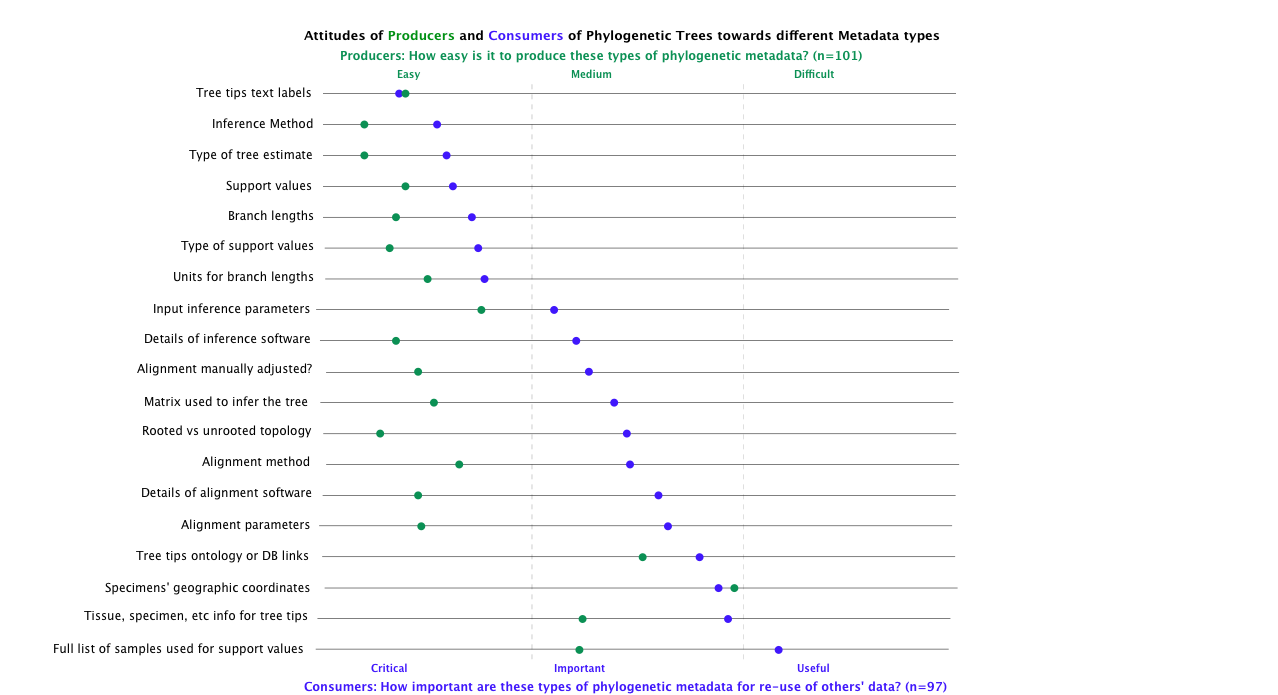
\includegraphics[width=3in]{rasters/OTOL graph - wide.png}
	\captionof{figure}{Caption}
	\label{label}
\end{Figure}

\section{Discussion}


\section{Conclusion}

%Bibliography note: this is keyed to Elliott's Mendeley bib dump, so pass any added references to me for inclusion.  I'll export a purposive .bib file once we're done.
\bibliographystyle{apa}
\bibliography{BibTex}

\end{multicols}

\end{document}
